\documentclass{article}

\usepackage{booktabs}
\usepackage{tabularx}
\usepackage{caption}
\usepackage{bookmark}
\usepackage{enumitem}
\usepackage{hyperref}
\usepackage{graphicx}

% From: https://tex.stackexchange.com/questions/438876/how-to-cross-reference-text-with-a-custom-label-reference-text
\makeatletter
\newcommand{\labeltext}[3][]{%
    \@bsphack%
    \csname phantomsection\endcsname% in case hyperref is used
    \def\tst{#1}%
    \def\labelmarkup{\emph}% How to markup the label itself
    %\def\refmarkup{\labelmarkup}% How to markup the reference
    \def\refmarkup{}%
    \ifx\tst\empty\def\@currentlabel{\refmarkup{#2}}{\label{#3}}%
    \else\def\@currentlabel{\refmarkup{#1}}{\label{#3}}\fi%
    \@esphack%
    \labelmarkup{#2}% visible printed text.
}
\makeatother

\title{Software Requirements Specification: Realm\\\progname}

\author{\authname}

\date{}

%% Comments

\usepackage{color}

\newif\ifcomments\commentstrue %displays comments
%\newif\ifcomments\commentsfalse %so that comments do not display

\ifcomments
\newcommand{\authornote}[3]{\textcolor{#1}{[#3 ---#2]}}
\newcommand{\todo}[1]{\textcolor{red}{[TODO: #1]}}
\else
\newcommand{\authornote}[3]{}
\newcommand{\todo}[1]{}
\fi

\newcommand{\wss}[1]{\authornote{blue}{SS}{#1}} 
\newcommand{\plt}[1]{\authornote{magenta}{TPLT}{#1}} %For explanation of the template
\newcommand{\an}[1]{\authornote{cyan}{Author}{#1}}

%% Common Parts

\newcommand{\progname}{Software Engineering} % PUT YOUR PROGRAM NAME HERE
\newcommand{\authname}{Team \#13, ARC
    \\ Avanish, Ahluwalia
    \\ Russell, Davidson
    \\ Rafey, Malik
    \\ Abdul, Zulfiqar} % AUTHOR NAMES                  

\usepackage{hyperref}
    \hypersetup{colorlinks=true, linkcolor=blue, citecolor=blue, filecolor=blue,
                urlcolor=blue, unicode=false}
    \urlstyle{same}
                                


\begin{document}

\maketitle

\newpage{}

\tableofcontents

\addcontentsline{toc}{section}{Revision History}
\section*{Revision History}

\begin{table}[hp]
\caption{Revision History} \label{TblRevisionHistory}
\begin{tabularx}{\textwidth}{llX}
\toprule
\textbf{Date} & \textbf{Developer(s)} & \textbf{Change}\\
\midrule
2024-10-07 & Russell Davidson & \nameref{sub:compliance}, \nameref{ssub:installation}, \nameref{ssub:distribution}, and \nameref{ssub:portability} \\
2024-10-07 & Russell Davidson & \nameref{ssub:tutorial}, \nameref{ssub:tour_management}, and \nameref{ssub:touring} \\
2024-10-08 & Russell Davidson & \ref{uc:1}, \ref{uc:2}, \ref{uc:3}, and \ref{uc:4} \\
2024-10-10 & Russell Davidson & \ref{uc:26}, \ref{uc:27}, and \nameref{sub:use_cases} diagram\\
2024-10-11 & Russell Davidson & \ref{uc:4} sequence diagram\\
\bottomrule
\end{tabularx}
\end{table}

\section{Introduction}


\subsection{Document Purpose}


\subsection{Product Scope}


\subsection{Definitions, Acronyms and Abbreviations}
\label{sub:def_acr_abb}

\begin{itemize}
    \item \labeltext{AR object}{def:ar_obj}: A 2D/3D projection of an entity.
    \item \labeltext{Users}{def:user}: A term for anyone who uses the app.
    \item \labeltext{Organization users}{def:org_user}: Users who belong to an organization that has the ability to create tours. They are affiliated with a particular approved organization who have the ability to modify tours within their organization’s domain.
    \item \labeltext{General users}{def:gen_user}: Users that can access most of the app functionalities except creating tours.
    \item \labeltext{Admins}{def:admin}: People who have access to nothing else but the admin interface within the app.
\end{itemize}

\subsubsection{Screen Names}
\begin{itemize}
    \item \textbf{Realm screen:} the screen in the app that provides a view of AR objects imposed on a feed of the user’s camera.
    \item \textbf{Tour List screen:} Shows a list of the available tours and an option to start them.
    \item \textbf{Tour Editor screen:} Allows organization users to edit tours and publish changes.
    \item \textbf{Maps screen:} Map view displaying objects placed around you
    \item \textbf{Inventory:} A display of available AR objects (personal objects, objects mapped to a group and application preset objects)
    \begin{itemize}
        \item \textbf{Groups screen:} Ability to add, edit and interact with group settings
        \item \textbf{Friends screen:} Managing friends
        \item \textbf{Settings:} Accessibility settings, Display settings, Privacy settings, Profile Settings, Group settings
        \item \textbf{Help:} FAQ and request org account
    \end{itemize}
    \item \textbf{Placement Editor:} Able to move, rotate, resize the object prior to confirming placement.
\end{itemize}

\subsection{References}
\label{sub:references}

\begingroup
\raggedright
\bibliography{ref}
\endgroup
\bibliographystyle{ieeetr}

\subsection{Document Overview}


\section{Product Overview}


\subsection{Product Perspective}


\subsection{Product Functions}


\subsection{Product Constraints}

\subsection{User Characteristics}


\subsection{Assumptions and Dependencies}


\subsection{Apportioning of Requirements}


\section{Requirements}


\subsection{External Interfaces}

\subsubsection{User interfaces}

\begin{center}
    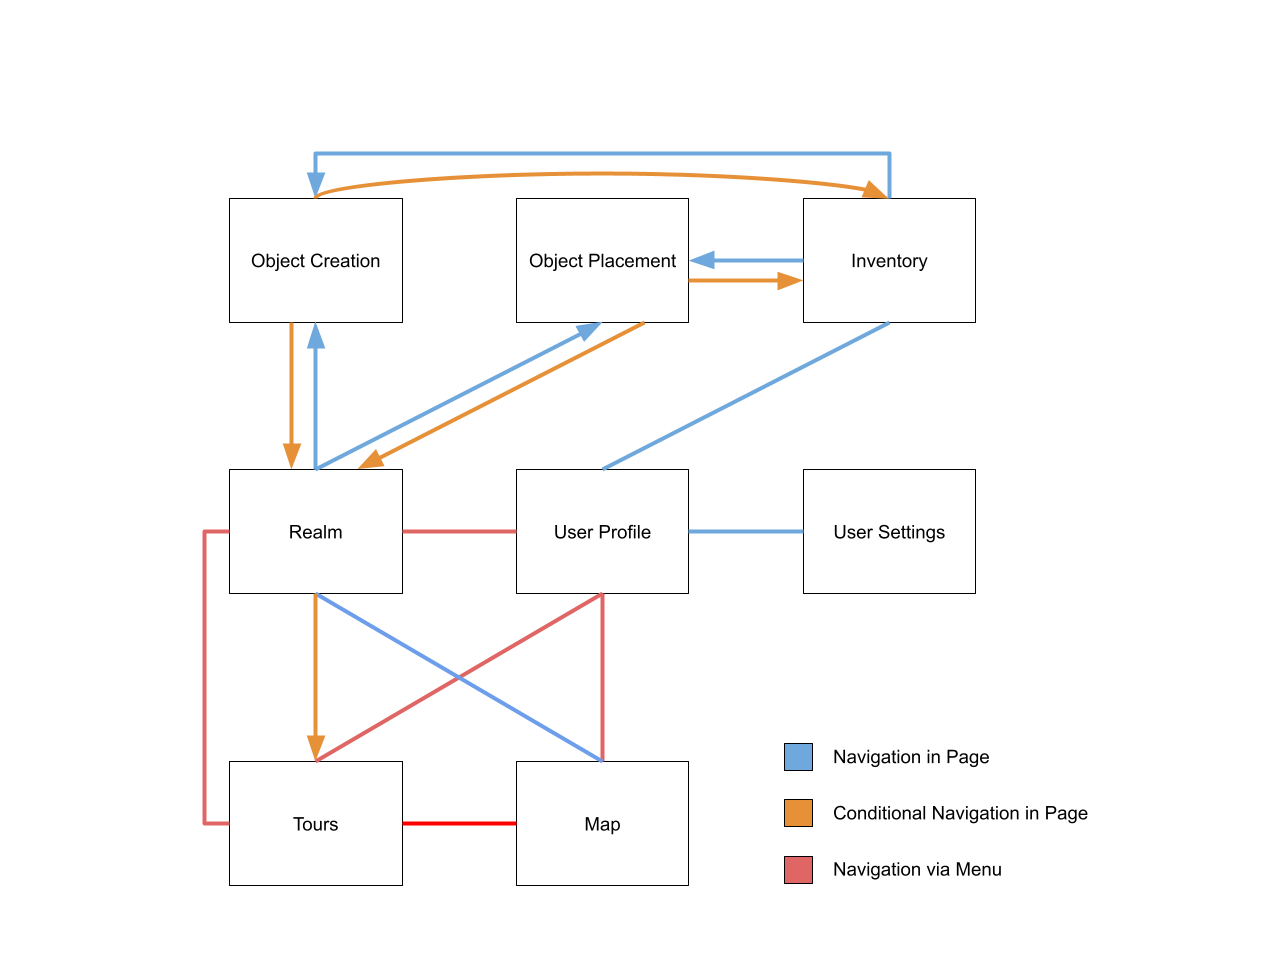
\includegraphics[scale=0.4]{OtherDiagrams/ui_flow.png}
\end{center}

There must be a navigation menu that can be accessed from any page that allows the user to navigate to any of the four main pages: Realm, User Profile, Tours, and Map

\subsubsection{Look and Feel Requirements}

\textbf{LF-NFR1}

\begin{itemize}
    \item Description: The Realm Screen must provide an immersive view of AR objects imposed on the real world, and must be minimally interrupted by other UI elements. 
    \item Fit Criteria: Permanent UI elements besides the camera feed should take no more than 10\% of the space on the screen.
\end{itemize}




\subsubsection{Hardware interfaces}

\begin{center}
    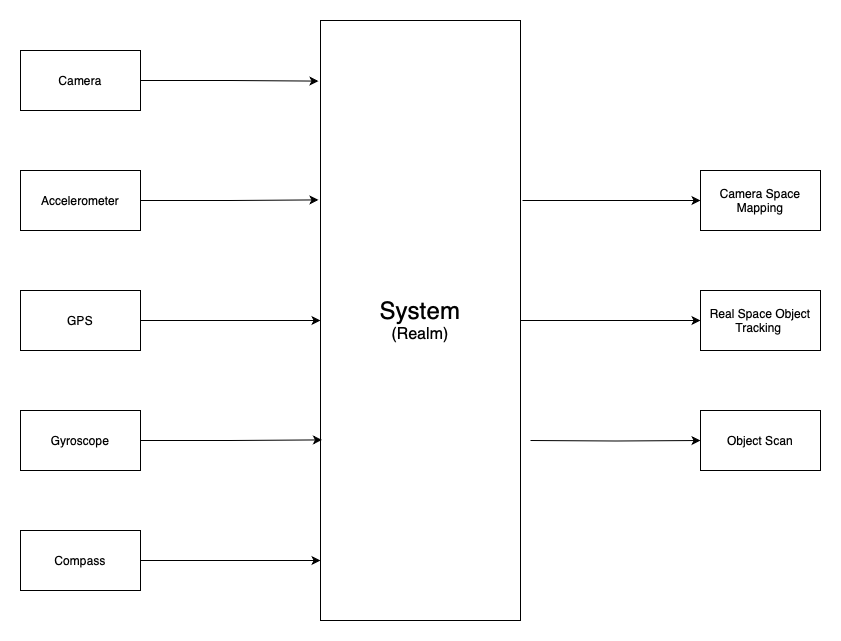
\includegraphics[scale=0.4]{OtherDiagrams/hscd.png}
\end{center}

The above figure shows the hardware inputs of the system and the outputs of the system that directly follow from the hardware inputs.


\subsubsection{Software interfaces}

\begin{center}
    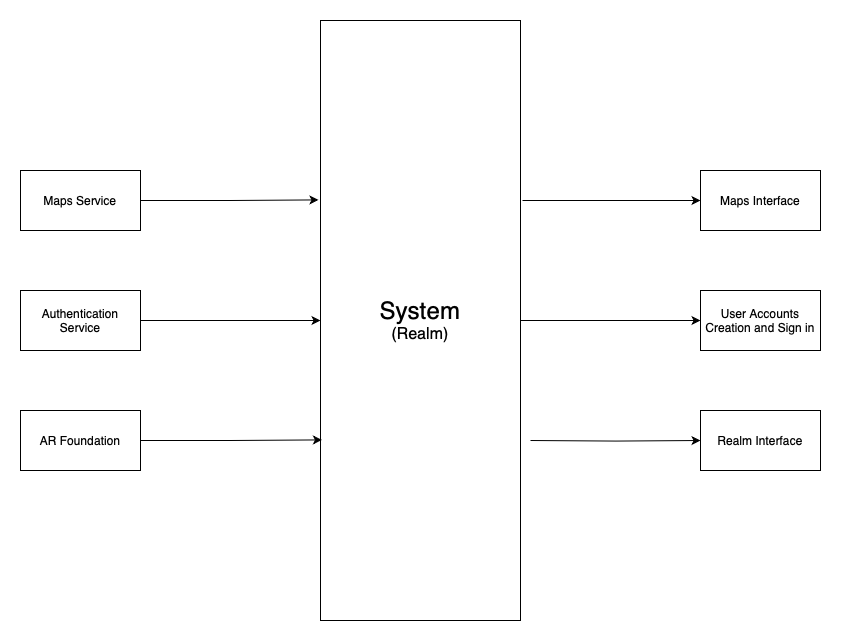
\includegraphics[scale=0.4]{OtherDiagrams/sscd.png}
\end{center}

The above figure shows the external systems our system will interact with, and the outputs of the system that directly follow from the external software inputs

\subsection{Functional}
\label{sub:functional}


\subsubsection{Tutorial}
\label{ssub:tutorial}

\begin{enumerate}[align=left, label=\textbf{TU-FR\arabic*:}]
    \item The app shall have a step-by-step interactive guide of how to use all major app features.
    \item The app shall prompt the user to complete the app tutorial after they create an account.
    \item The app shall allow the user to leave the tutorial at any time.
    \item The tutorial shall be available at any time through the app's help page in the \textbf{Settings screen}.
    \item The tutorial will involve user participation to directly use functionality in a sandbox environment.
\end{enumerate}

\begin{enumerate}[align=left, label=\textbf{TU-NFR\arabic*:}]
    \item Each interaction step should not take the user more than 15 seconds to figure out.
    \item The entire tutorial shall not take longer than 5 minutes to complete for 80\% of users.
\end{enumerate}

\subsubsection{Tour Management}
\label{ssub:tour_management}

\begin{enumerate}[align=left, label=\textbf{TM-FR\arabic*:}]
    \item The tour management functionality within the app shall only be available to \ref{def:org_user}.
    \item Tours within the app can be created as a “draft” to make it available to other \ref{def:org_user} but not released to the public.
    \item Tours within the app can be published to the public from a “draft” or from directly after creation.
    \item \ref{def:org_user} will be able to customize the following for each of their tours:
    \begin{enumerate}
        \item Name
        \item Description
        \item Route
        \begin{enumerate}
            \item Will be editable on a map of the tour area
            \item Intended direction of travel can be set
            \item Estimated time of completion that will be automatically determined by the distance if not set
        \end{enumerate}
        \item Objects
        \begin{enumerate}
            \item \ref{def:ar_obj} can be placed along the route at specific geographic locations along with description text for each of the \ref{def:ar_obj}
            \item Historical information text popups can be placed along the route
            \item All text will have an audio playback option with text-to-speech or pre-recorded audio (if available)
        \end{enumerate}
        \item Price
        \begin{enumerate}
            \item Can be free or
            \item a price under \$10
        \end{enumerate}
        \item Relevant Web Link(s)
    \end{enumerate}
    \item \ref{def:org_user} will have the ability to preview the tours that belong to their organization.
    \item \ref{def:org_user} will have the ability to edit tours that belong to their organization.
\end{enumerate}

\subsubsection{Touring}
\label{ssub:touring}

\begin{enumerate}[align=left, label=\textbf{TR-FR\arabic*:}]
    \item The touring functionality within the app shall only be available to \ref{def:gen_user}.
    \item The app will have three avenues for a user to find tours:
    \begin{enumerate}[align=left, label=\textbf{TR-FR2.\arabic*:}]
        \item The app will allow \ref{def:gen_user} to see a list of available tours through the \textbf{Tour List Interface}.
        \begin{itemize}
            \item The tours can be grouped in this page by organization or by location
        \end{itemize}
        \item The app will also have tours show up in a push notification (if configured by a user) when in close proximity to a tour area.
        \item Locations can place QR codes at the starting location of the tour which can be scanned by a mobile camera that will open the tour preview in the app.
    \end{enumerate}
    \item Users will be able to preview a tour to see the following information:
    \begin{enumerate}
        \item Name
        \item Description
        \item Relevant web link(s)
        \item Tour distance (auto-calculated from route)
        \item Estimated time of completion
        \item A map that will show the route and locations of \ref{def:ar_obj}s
        \item Price
    \end{enumerate}
    \item Once a user starts a tour they will have two main views they can switch between:
    \begin{enumerate}[align=left, label=\textbf{TR-FR4.\arabic*:}]
        \item One of the tour views is a map
        \begin{itemize}
            \item The designated tour area will be outlined
            \item The user’s current location will be shown
            \item Intended route and direction will be overlaid
            \item Location of \ref{def:ar_obj}s will be marked
        \end{itemize}
        \item One of the tour views is an AR view
        \begin{itemize}
            \item Will be very similar to the interface of the \textbf{Realm Interface}
            \item Have an added indicator of the intended direction
            \item Popups for historical information
        \end{itemize}
    \end{enumerate}
\end{enumerate}

\subsubsection{Object Placement}
\label{ssub:object_placement}

\begin{enumerate}[align=left, label=\textbf{OP-FR\arabic*:}]
    \item The system must have the capability to store object instances that specify the following details:
    \begin{itemize}
        \item The AR object that was placed.
        \item The sub-realm(s) in which the object instance will be shared.
        \item All data required to precisely reproduce the position and orientation of the object in real space.
    \end{itemize}
    
    \item The system must provide a way for a user to place AR objects in the space around them, creating object instances.
    \begin{enumerate}[align=left, label=\textbf{OP-FR2.\arabic*:}]
        \item The system must provide a way for a user to select an object either from their inventory or by generating a new object.
        \item The system must provide a way for the user to select one or more sub-realms of which they are a member.
        \item The system must provide a way for the user to position an AR object in real space.
    \end{enumerate}
\end{enumerate}

\subsubsection{Realm Interface}
\label{ssub:realm_interface}

\begin{enumerate}[align=left, label=\textbf{RI-FR\arabic*:}]
    \item The Realm interface must provide a view of the AR object instances in the area around the user overlaid on their camera feed positioned in real space.
    \begin{enumerate}[align=left, label=\textbf{RI-FR1.\arabic*:}]
        \item AR object instances presented on the Realm interface must always appear to change perspective correctly with respect to the user’s camera position and angle.
        \item AR object instances that overlap or clutter a given area in real space will not be presented simultaneously.
        \item AR object instances reproduced on the Realm interface must be in the correct position and orientation as defined by the object placement.
    \end{enumerate}
    
    \item The Realm interface must keep track of a selected sub-realm which determines which object instances are displayed.
    \begin{enumerate}[align=left, label=\textbf{RI-FR2.\arabic*:}]
        \item The Realm interface must provide an indication of what sub-realm is currently selected.
        \item The Realm interface must provide a way for the user to change the selected sub-realm.
    \end{enumerate}
    
    \item The Realm interface must provide a control to allow the user to enter the object placement workflow. 
    \item The Realm interface must provide a control to allow the user to enter the object scanning workflow.
    \item When the user is near the starting point of a tour, the Realm interface must provide an indication that there is a tour nearby as well as a link to the tour preview.
\end{enumerate}


\subsubsection{Admin Interface}
\label{ssub:admin_interface}

\begin{enumerate}[align=left, label=\textbf{AI-FR\arabic*:}]
    \item The admin interface within the app shall only be available to \ref{def:admin}.
    \item The app shall provide an interface for \ref{def:admin} to carry-out their two special roles:
    \begin{enumerate}[align=left, label=\textbf{AI-FR2.\arabic*:}]
        \item The app shall permit \ref{def:admin} to act on user reports of an \ref{def:ar_obj} by either keeping or removing the \ref{def:ar_obj}.
        \item The app shall permit \ref{def:admin} to review requests for \ref{def:org_user} accounts and either accept or deny the request.
    \end{enumerate}
\end{enumerate}

\subsection{Use Cases}
\label{sub:use_cases}

\begin{center}
    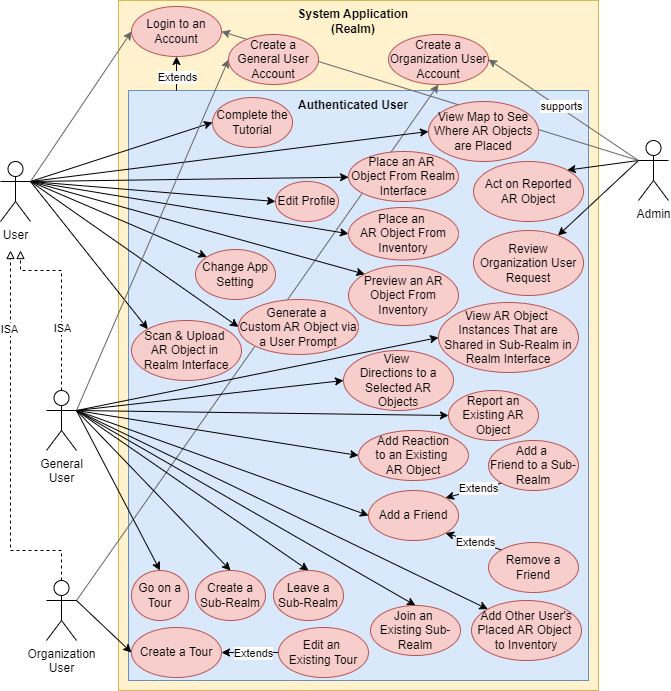
\includegraphics[scale=0.5]{use_cases.png}\\ 
    \textbf{Figure 1: Use Cases}
\end{center}

\begin{enumerate}[label=\textbf{UC\arabic*}]
    \item \label{uc:1} Complete the Tutorial \\
        \textbf{Actor}: \ref{def:user} \\
        \textbf{Pre-condition:} User has opened the app \\
    
        \textbf{Main Success Scenario:}
        \begin{enumerate}[label=\textbf{\arabic*.}]
            \item User creates an account (\ref{uc:23})
            \item System prompts user to complete the tutorial (\hyperref[ssub:tutorial]{TU-FR2})
            \item User indicates they would like to do the tutorial
            \item System opens the \textbf{Tutorial Interface}
            \item System provides directions to use a feature
            \item User tries the feature (\hyperref[ssub:tutorial]{TU-FR5})
            \item User goes to next feature when satisfied
            \item Repeat steps \textbf{5}-\textbf{7} for all major app features (\hyperref[ssub:tutorial]{TU-FR1})
            \item System prompts user to leave and end tutorial
            \item User ends tutorial (\hyperref[ssub:tutorial]{TU-FR3})
            \item System redirects to \textbf{Home Interface}
        \end{enumerate}
    
        \textbf{Secondary Scenarios:} 
        \begin{itemize}
            \item[{\bf 1.1:}] User already has an account
            \begin{enumerate}[label=\textbf{\arabic*.}]
                \item User logs into account (\ref{uc:24})
                \item User navigates to \textbf{Help Interface} (\hyperref[ssub:tutorial]{TU-FR4})
                \item Go to step \textbf{2}
            \end{enumerate}
            \item[{\bf 10.1:}] User chooses to stay in sandbox environment
            \begin{enumerate}[label=\textbf{\arabic*.}]
                \item System closes prompt and allows user to use sandbox environment
                \item User indicates they want to leave tutorial
                \item Go to step \textbf{11}
            \end{enumerate}
        \end{itemize}
        \textbf{Success Postcondition:} The user has a general idea of how all the app’s major features work.

    \item \label{uc:2} Create a Tour \\
        \textbf{Actor}: \ref{def:org_user} \\
        \textbf{Pre-condition:} User is logged into the app \textbf{AND} User has navigated to the \textbf{Tour Management Interface} \\
    
        \textbf{Main Success Scenario:}
        \begin{enumerate}[label=\textbf{\arabic*.}]
            \item User selects the option to create a new tour
            \item System opens up a form for the user to add the following information about the tour (\hyperref[ssub:tour_management]{TM-FR4[1,2,5,6]}):
            \begin{enumerate}
                \item Name
                \item Description
                \item Price
                \item Relevant web link(s)
            \end{enumerate}
            \item User fills out the information
            \item System identifies no blank fields
            \item System gives the option to move on to the route configuration
            \item User goes to the route configuration
            \item System presents tour route configuration
            \item User configures tour area, route, and direction (\hyperref[ssub:tour_management]{TM-FR4[3]})
            \item System gives the option to move on to the inventory setup
            \item User goes to the inventory setup (\hyperref[ssub:tour_management]{TM-FR4[4]})
            \item System opens the \textbf{Inventory Interface}
            \item User scans and uploads a new \ref{def:ar_obj} (\ref{uc:5})
            \item User repeats step \textbf{12} until all desired \ref{def:ar_obj}s are uploaded
            \item User indicates they would like to move on to object placement
            \item System opens the \textbf{Realm Interface} and allows the user to place \ref{def:ar_obj}s and historical information popups in an isolated environment.
            \item User places down \ref{def:ar_obj} using the \textbf{Realm Interface} (\ref{uc:7})
            \item User repeats step \textbf{16} until all desired \ref{def:ar_obj}s are placed
            \item User indicates they would like to finish tour creation
            \item System gives the user the option create the tour as a draft or directly publish it (\hyperref[ssub:tour_management]{TM-FR2/TM-FR3})
            \item User selects direct publish option
            \item System uploads the tour data
            \item System makes the tour available to \ref{def:gen_user}
        \end{enumerate}
    
        \textbf{Secondary Scenarios:} 
        \begin{itemize}
            \item[{\bf 4.1:}] System identifies some blank fields
            \begin{enumerate}[label=\textbf{\arabic*.}]
                \item System validates input to ensure all required fields are not empty
                \item System determines input passes validation
                \item Go to step \textbf{5}
            \end{enumerate}
            \item[{\bf 4.1.2:}] System determines input fails validation
            \begin{enumerate}[label=\textbf{\arabic*.}]
                \item Go to step \textbf{3}
            \end{enumerate}
            \item[{\bf 12.1:}] User does not have any \ref{def:ar_obj}s to scan
            \begin{enumerate}[label=\textbf{\arabic*.}]
                \item Go to step \textbf{14}
            \end{enumerate}
            \item[{\bf 20.1:}] User selects draft option
            \begin{enumerate}[label=\textbf{\arabic*.}]
                \item System uploads the tour data but does not make it available to \ref{def:gen_user}
                \item User decides at a later time to publish the draft tour
                \item Go to step \textbf{22}
            \end{enumerate}
        \end{itemize}
        \textbf{Success Postcondition:} One of the \ref{def:org_user} has a new tour linked to their organization

    \item \label{uc:3} Edit an existing Tour \\
        \textbf{Actor}: \ref{def:org_user} \\
        \textbf{Pre-condition:} User is logged into the app \textbf{AND} User has at least one tour connected to their organization \textbf{AND} User has navigated to the \textbf{Tour Management Interface} \\
    
        \textbf{Main Success Scenario:}
        \begin{enumerate}[label=\textbf{\arabic*.}]
            \item System provides a list of all tours connected to the user’s organization
            \item User selects one of the tours
            \item System shows the preview of the tour (\hyperref[ssub:tour_management]{TM-FR5})
            \item System provides the option to edit the tour (\hyperref[ssub:tour_management]{TM-FR6})
            \item User decides to edit the tour
            \item System opens up a form for the user to with the following information about the tour that may or not be populated (\hyperref[ssub:tour_management]{TM-FR4[1,2,5,6]}):
            \begin{enumerate}
                \item Name
                \item Description
                \item Price
                \item Relevant web link(s)
            \end{enumerate}
            \item User edits information as desired
            \item System identifies no blank fields
            \item System gives the option to move on to the route configuration
            \item User goes to the route configuration
            \item System presents tour route configuration
            \item User edits configuration of tour area, route, and direction as desired (\hyperref[ssub:tour_management]{TM-FR4[3]})
            \item System gives the option to move on to the inventory setup
            \item User goes to the inventory setup (\hyperref[ssub:tour_management]{TM-FR4[4]})
            \item System opens the \textbf{Inventory Interface}
            \item User scans and uploads a new \ref{def:ar_obj} (\ref{uc:5})
            \item User repeats step \textbf{12} until all desired \ref{def:ar_obj}s are uploaded
            \item User indicates they would like to move on to object placement
            \item System opens the \textbf{Realm Interface} and allows the user to place/edit \ref{def:ar_obj}s and historical information popups in an isolated environment.
            \item User edits \ref{def:ar_obj} using the \textbf{Realm Interface} (\ref{uc:7})
            \item User repeats step \textbf{16} until all desired \ref{def:ar_obj}s are edited
            \item User indicates they would like to finish tour editing
            \item System gives the user the option to save the edited tour as a draft or directly publish it (\hyperref[ssub:tour_management]{TM-FR2/TM-FR3})
            \item User selects direct publish option
            \item System uploads the updated tour data
            \item System makes the updated tour available to \ref{def:gen_user}
        \end{enumerate}
    
        \textbf{Secondary Scenarios:} 
        \begin{itemize}
            \item[{\bf 5.1:}] User decides not to edit the tour
            \begin{enumerate}[label=\textbf{\arabic*.}]
                \item System goes back to the \textbf{Tour Management Interface}
            \end{enumerate}
            \item[{\bf 8.1:}] System identifies some blank fields
            \begin{enumerate}[label=\textbf{\arabic*.}]
                \item System validates input to ensure all required fields are not empty
                \item System determines input passes validation
                \item Go to step \textbf{9}
            \end{enumerate}
            \item[{\bf 16.1:}] User decides not to scan and upload any new \ref{def:ar_obj}s
            \begin{enumerate}[label=\textbf{\arabic*.}]
                \item Go to step \textbf{18}
            \end{enumerate}
            \item[{\bf 20.1:}] User places down new \ref{def:ar_obj} using the \textbf{Realm Interface}
            \begin{enumerate}[label=\textbf{\arabic*.}]
                \item User repeats step \textbf{20.1} until all desired \ref{def:ar_obj}s are placed
            \end{enumerate}
            \item[{\bf 24.1:}] User selects draft option
            \begin{enumerate}[label=\textbf{\arabic*.}]
                \item System uploads the updated tour data but does not make it available to \ref{def:gen_user}
                \item User decides at a later time to publish the draft of the updated tour
                \item Go to step \textbf{26}
            \end{enumerate}
        \end{itemize}
        \textbf{Success Postcondition:} One of the \ref{def:org_user} has edited an existing tour linked to their organization

    \item \label{uc:4} Go on a tour \\
        \textbf{Actor}: \ref{def:gen_user} \\
        \textbf{Pre-condition:} User is logged into the app \\
    
        \textbf{Main Success Scenario:}
        \begin{enumerate}[label=\textbf{\arabic*.}]
            \item User navigates to the \textbf{Tour Interface}
            \item System displays a list of all tours
            \item User selects a tour (\hyperref[ssub:touring]{TR-FR2.1})
            \item System opens up the preview of the selected tour (\hyperref[ssub:touring]{TR-FR3})
            \item System also provides the option to take the tour
            \item User reviews details of the tour
            \item User decides to go on the tour
            \item System opens a modified version of the \textbf{Realm Interface} in an isolated environment that does not allow them to place any objects or modify existing objects (\hyperref[ssub:touring]{TR-FR4.2})
            \item System shows the intended direction of travel
            \item User walks to the highlighted \ref{def:ar_obj} of interest
            \item System acknowledges when the user makes it to the \ref{def:ar_obj}
            \item System provides historical information regarding \ref{def:ar_obj}
            \item System updates the target to be the next \ref{def:ar_obj}
            \item Repeat steps \textbf{10}-\textbf{13} for every \ref{def:ar_obj}
            \item System indicates that the tour has been completed
            \item System provides metrics for time taken and distance traveled
            \item System prompts user to leave tour
            \item User leaves tour
            \item System goes back to the tour list
        \end{enumerate}
    
        \textbf{Secondary Scenarios:} 
        \begin{itemize}
            \item[{\bf 1.1:}] System pushes a notification to the user when they are in the proximity of a tour (\hyperref[ssub:touring]{TR-FR2.2})
            \begin{enumerate}[label=\textbf{\arabic*.}]
                \item System opens up the \textbf{Tour Interface}
                \item Go to step \textbf{4}
            \end{enumerate}
            \item[{\bf 1.2:}] User scans a tour QR code in camera app (\hyperref[ssub:touring]{TR-FR2.3})
            \begin{enumerate}[label=\textbf{\arabic*.}]
                \item System opens up the \textbf{Tour Interface}
                \item Go to step \textbf{4}
            \end{enumerate}
            \item[{\bf 7.1:}] User decides not to go on the tour
            \begin{enumerate}[label=\textbf{\arabic*.}]
                \item Go to step \textbf{19}
            \end{enumerate}
            \item[{\bf 10.1:}] User indicates they want to open the map
            \begin{enumerate}[label=\textbf{\arabic*.}]
                \item System opens up the \textbf{Map} view of the tour (\hyperref[ssub:touring]{TR-FR4.2})
                \item System shows the user’s current location
                \item System shows the indented route, direction and boundaries of the tour
                \item System marks the location of \ref{def:ar_obj}s
                \item User views the map
                \item User closes the map
                \item Go to step \textbf{9}
            \end{enumerate}
            \item[{\bf 14.1:}] User does not want to go to all \ref{def:ar_obj}s
            \begin{enumerate}[label=\textbf{\arabic*.}]
                \item User indicates they wish to exit the tour
                \item Go to step \textbf{19}
            \end{enumerate}
            \item[{\bf 18.1:}] User does not leave tour
            \begin{enumerate}[label=\textbf{\arabic*.}]
                \item System removes target object and allows user to explore \ref{def:ar_obj}s in the isolated environment
                \item User eventually decides to exit the tour
                \item Go to step \textbf{19}
            \end{enumerate}
        \end{itemize}
        \textbf{Success Postcondition:} One of the \ref{def:gen_user} has completed a tour
    
    \item \label{uc:7} Place an AR object from the \textbf{Realm Interface} (\hyperref[ssub:realm_interface]{RI-FR1}) \\ 
        \textbf{Actor}: General User \\ 
        \textbf{Pre-condition:} User is logged in to the app \textbf{AND} has navigated to the \textbf{Realm Interface} (\hyperref[ssub:realm_interface]{RI-FR1}) \\
    
        \textbf{Main Success Scenario:}
        \begin{enumerate}[label=\textbf{\arabic*.}]
            \item System presents \textbf{Realm interface}.
            \item User performs control to initiate object placement.
            \item System presents the \textbf{Object Selection Menu} (\hyperref[ssub:object_placement]{OP-FR2.1}).
            \item User selects an existing AR object for placement.
            \item System presents the \textbf{Sub-Realm Selection Menu} (\hyperref[ssub:object_placement]{OP-FR2.2}).
            \item User selects the sub-realm(s) in which they wish for their object instance to be shared.
            \item System presents the \textbf{Object Positioning Interface} (\hyperref[ssub:object_placement]{OP-FR2.3}). 
            \item User positions the AR object using given controls and confirms when done.
            \item System returns to Realm screen.
        \end{enumerate}
    
        \textbf{Secondary Scenarios:}
        \begin{itemize}
            \item[{\bf 3.1:}] User creates new object with a prompt:
            \begin{enumerate}[label=\textbf{\arabic*.}]
                \item Main scenario steps 1-3.
                \item User selects the option to generate an object via prompt.
                \item System presents the \textbf{Prompt Object Generation Interface}.
                \item User completes the prompt object generation workflow.
                \item Main scenario steps 5-9.
            \end{enumerate}
    
            \item[{\bf 3.2:}] User creates a new object with object scanning:
            \begin{enumerate}[label=\textbf{\arabic*.}]
                \item Main scenario steps 1-3.
                \item User selects the option to generate an object via object scan.
                \item System presents the \textbf{Object Scanning Interface}.
                \item User completes object scanning workflow.
                \item Main scenario steps 5-9.
            \end{enumerate}
    
            \item[{\bf 3.3, 5.1, 7.1:}] User cancels object placement:
            \begin{enumerate}[label=\textbf{\arabic*.}]
                \item Main scenario steps 1-3, or 1-5, or 1-7.
                \item User selects option to cancel object placement.
                \item System returns to the \textbf{Realm Interface}.
            \end{enumerate}
    
            \item[{\bf 5.1:}] User reselects object:
            \begin{enumerate}[label=\textbf{\arabic*.}]
                \item Main scenario steps 1-5.
                \item User selects option to return to \textbf{Object Selection Menu} (\hyperref[ssub:object_placement]{OP-FR2.1}).
                \item Main scenario resumes from step 3.
            \end{enumerate}
    
            \item[{\bf 7.2:}] User reselects Sub-realms:
            \begin{enumerate}[label=\textbf{\arabic*.}]
                \item Main scenario steps 1-7.
                \item User selects option to return to \textbf{Sub-Realm Selection Menu} (\hyperref[ssub:object_placement]{OP-FR2.2}).
                \item Main scenario resumes from step 5.
            \end{enumerate}
        \end{itemize}
    
        \textbf{Success Postcondition:} Users that are members of the sub-realm in which the object instance has been shared can see the object instance from the \textbf{Realm interface}.
    
    \item \label{uc:8} Place an AR object from the Inventory \\ 
        \textbf{Actor}: General User \\ 
        \textbf{Pre-condition:} User is logged in to the app \textbf{AND} has navigated to the \textbf{Inventory Interface} \\
    
        \textbf{Main Success Scenario:}
        \begin{enumerate}[label=\textbf{\arabic*.}]
            \item System presents Inventory interface.
            \item User selects an object they wish to place.
            \item System presents object details.
            \item User selects option to initiate object placement.
            \item System presents the \textbf{Sub-Realm Selection Menu} (\hyperref[ssub:object_placement]{OP-FR2.1}).
            \item User selects the sub-realm(s) in which they wish for their object instance to be shared.
            \item System presents the \textbf{Object Positioning Interface} (\hyperref[ssub:object_placement]{OP-FR2.3}).
            \item User positions the AR object using given controls and confirms when done.
            \item System returns to Realm screen.
        \end{enumerate}
    
        \textbf{Secondary Scenarios:}
        \begin{itemize}
            \item[{\bf 5.1, 7.1:}] User cancels object placement:
            \begin{enumerate}[label=\textbf{\arabic*.}]
                \item Main scenario steps 1-5, or 1-7.
                \item User selects option to cancel object placement.
                \item System returns to the Inventory screen.
            \end{enumerate}
    
            \item[{\bf 7.2:}] User reselects Sub-realm:
            \begin{enumerate}[label=\textbf{\arabic*.}]
                \item Main scenario steps 1-7.
                \item User selects option to return to \textbf{Sub-Realm Selection} (\hyperref[ssub:object_placement]{OP-FR2.2}).
                \item Main scenario resumes from step 5.
            \end{enumerate}
        \end{itemize}
    
        \textbf{Success Postcondition:} Users that are members of the sub-realm in which the object instance has been shared can see the object instance from the \textbf{Realm Interface}.
    
    \item \label{uc:10} View object instances that are shared in a Sub-realm in the \textbf{Realm interface} \\ 
        \textbf{Actor}: General User \\ 
        \textbf{Pre-condition:} User is logged in to the app \textbf{AND} has navigated to the \textbf{Realm Interface} (\hyperref[ssub:realm_interface]{RI-FR1}) \\
    
        \textbf{Main Success Scenario:}
        \begin{enumerate}[label=\textbf{\arabic*.}]
            \item System presents the \textbf{Realm Interface}.
            \item User selects a sub-realm to see objects from.
            \item System only presents object instances in the selected sub-realm.
            \item User moves their device to see any angle of the object instance.
            \item System continuously presents the object instance with the correct perspective relative to the user’s camera.
        \end{enumerate}
    
        \textbf{Secondary Scenarios:}
        \begin{itemize}
            \item[{\bf 10.1:}] User is not a member of any sub-realms:
            \begin{enumerate}[label=\textbf{\arabic*.}]
                \item System presents \textbf{Realm Interface} (\hyperref[ssub:realm_interface]{RI-FR1}).
                \item System presents only public object instances.
                \item User moves their device to see any angle of the object instance.
                \item System continuously presents the object instance with the correct perspective relative to the user’s camera.
            \end{enumerate}
        \end{itemize}
    
        \textbf{Success Postcondition:} The user can see any AR object instances that are in any sub-realm that they are a part of correctly positioned in real space.

    \item \label{uc:14} Report an existing AR object \\ 
        \textbf{Actor}: General User \\ 
        \textbf{Pre-condition:} User is logged in to the app \textbf{AND} has navigated to the \textbf{Realm Interface} (\hyperref[ssub:realm_interface]{RI-FR1}) \textbf{AND} there is another user’s AR object placed in the vicinity of the user \\

        \textbf{Main Success Scenario:}
        \begin{enumerate}[label=\textbf{\arabic*.}]
            \item System presents \textbf{Realm Interface} with another user’s object instance present on screen.
            \item User selects the object they wish to report from the screen.
            \item System presents \textbf{Object Selection Context Action Menu}.
            \item User selects option to report object.
            \item System presents \textbf{Object Reporting Interface}.
            \item User provides required details for report and submits report.
            \item System presents message thanking user for report.
        \end{enumerate}

        \textbf{Secondary Scenarios:}
        \begin{itemize}
            \item[{\bf 5.1:}] User cancels report:
            \begin{enumerate}[label=\textbf{\arabic*.}]
                \item User closes \textbf{Object Reporting Interface}.
                \item System returns to \textbf{Realm Interface}.
            \end{enumerate}

            \item[{\bf 3.1:}] User cancels object selection:
            \begin{enumerate}[label=\textbf{\arabic*.}]
                \item User closes \textbf{Object Selection Context Action Menu}.
                \item Main scenario resumes from step 2.
            \end{enumerate}
        \end{itemize}

        \textbf{Success Postcondition:} The user is informed that their report will be investigated. The system initiates a report review process.

    \item \label{uc:15} Add reaction to an existing AR object instance \\ 
        \textbf{Actor}: General User \\ 
        \textbf{Pre-condition:} User is logged in to the app \textbf{AND} has navigated to the \textbf{Realm Interface} (\hyperref[ssub:realm_interface]{RI-FR1}) \textbf{AND} there is an AR object placed in the vicinity of the user \\

        \textbf{Main Success Scenario:}
        \begin{enumerate}[label=\textbf{\arabic*.}]
            \item System presents \textbf{Realm Interface} with an object instance present on screen.
            \item User selects the object they wish to react to from the screen.
            \item System presents \textbf{Object Selection Context Action Menu}.
            \item User selects option to react to object instance.
            \item System presents \textbf{Reaction Selection Menu}.
            \item User selects desired reaction.
            \item System returns to \textbf{Object Selection Context Action Menu} with user reaction displayed.
        \end{enumerate}

        \textbf{Secondary Scenarios:}
        \begin{itemize}
            \item[{\bf 3.1:}] User cancels object selection:
            \begin{enumerate}[label=\textbf{\arabic*.}]
                \item User closes \textbf{Object Selection Context Action Menu}.
                \item Main scenario resumes from step 2.
            \end{enumerate}
        \end{itemize}

        \textbf{Success Postcondition:} The user’s reaction is visible to any user who selects the AR object instance.

    \item \label{uc:16} Add other user’s placed AR object to Inventory \\ 
        \textbf{Actor}: General User \\ 
        \textbf{Pre-condition:} User is logged in to the app \textbf{AND} has navigated to the \textbf{Realm Interface} (\hyperref[ssub:realm_interface]{RI-FR1}) \textbf{AND} there are other users’ AR objects placed in the vicinity of the user \\

        \textbf{Main Success Scenario:}
        \begin{enumerate}[label=\textbf{\arabic*.}]
            \item System presents \textbf{Realm Interface} with another user’s object instance present on screen.
            \item User selects the object they wish to add to their inventory from the screen.
            \item System presents \textbf{Object Selection Context Action Menu}.
            \item User selects option to add object to inventory.
            \item System returns to \textbf{Realm Interface} with indication that object has been added to Inventory.
        \end{enumerate}

        \textbf{Secondary Scenarios:}
        \begin{itemize}
            \item[{\bf 4.1:}] User inventory is full:
            \begin{enumerate}[label=\textbf{\arabic*.}]
                \item System returns to \textbf{Realm Interface} with indication that Inventory is full.
            \end{enumerate}

            \item[{\bf 3.1:}] User cancels object selection:
            \begin{enumerate}[label=\textbf{\arabic*.}]
                \item User exits \textbf{Object Selection Context Action Menu}.
                \item System returns to \textbf{Realm Interface}.
            \end{enumerate}
        \end{itemize}

        \textbf{Success Postcondition:} The user’s desired object is available in the user’s inventory for preview and placement.

    \item \label{uc:26}  Act on reported \ref{def:ar_obj} \\
        \textbf{Actor}: \ref{def:admin} \\
        \textbf{Pre-condition:} Admin is logged into the app \textbf{AND} Admin has navigated to the \textbf{Admin Interface} \\
    
        \textbf{Main Success Scenario:}
        \begin{enumerate}[label=\textbf{\arabic*.}]
            \item Admin navigates to the “AR Object Reports” panel (\hyperref[ssub:admin_interface]{AI-FR2.1})
            \item System shows a list of app \ref{def:ar_obj}s that have been reported
            \item Admin selects an object
            \item System gives more detailed information of \ref{def:ar_obj} and allows Admin to open an \ref{def:ar_obj} inventory preview (\hyperref[ssub:inventory]{IV-FR6})
            \item System also provides decision options on whether to keep the object or remove it
            \item Admin opens \ref{def:ar_obj} preview
            \item System shows preview of \ref{def:ar_obj}
            \item Admin views \ref{def:ar_obj} preview
            \item Admin closes \ref{def:ar_obj} preview
            \item System once again shows the object detailed information and decision options
            \item Admin reviews the information and decides to keep the \ref{def:ar_obj}
            \item System keeps \ref{def:ar_obj}
            \item System removes user report of \ref{def:ar_obj}
            \item System brings admin back to “AR Object Reports” panel
        \end{enumerate}
    
        \textbf{Secondary Scenarios:} 
        \begin{itemize}
            \item[{\bf 5.1:}] Admin does not open \ref{def:ar_obj} preview
            \begin{enumerate}[label=\textbf{\arabic*.}]
                \item Go to step \textbf{11}
            \end{enumerate}
            \item[{\bf 11.1:}] Admin reviews the information and decides to remove the object
            \begin{enumerate}[label=\textbf{\arabic*.}]
                \item System removes object
                \item Go to step \textbf{13}
            \end{enumerate}
        \end{itemize}
        \textbf{Success Postcondition:} An \ref{def:ar_obj} report is resolved (\ref{def:ar_obj} is kept or removed)

    \item \label{uc:27}  Act on reported \ref{def:ar_obj} \\
        \textbf{Actor}: \ref{def:admin} \\
        \textbf{Pre-condition:} Admin is logged into the app \textbf{AND} Admin has navigated to the \textbf{Admin Interface} \\
    
        \textbf{Main Success Scenario:}
        \begin{enumerate}[label=\textbf{\arabic*.}]
            \item Admin navigates to the “Organization User Requests” panel (\hyperref[ssub:admin_interface]{AI-FR2.2})
            \item System shows a list of \ref{def:org_user} requests
            \item Admin selects a request
            \item System gives more details about a request
            \item System also provides decision options on whether to accept or decline a request
            \item Admin reviews information and approves the request
            \item System activates the user as one of the \ref{def:org_user}
            \item System notifies the user that their request has been approved
            \item System removes organization user request
            \item System brings admin back to “Organization User Requests” panel
        \end{enumerate}
    
        \textbf{Secondary Scenarios:} 
        \begin{itemize}
            \item[{\bf 6.1:}] Admin reviews information and denies the request
            \begin{enumerate}[label=\textbf{\arabic*.}]
                \item System notifies the user that their request has been denied and gives a reason why
                \item Go to step \textbf{9}
            \end{enumerate}
        \end{itemize}
        \textbf{Success Postcondition:} An \ref{def:org_user} account request is resolved (approved or denied).
    
\end{enumerate}

\subsection{Quality of Service}

\subsubsection{Performance}


\subsubsection{Security}


\subsubsection{Reliability}


\subsubsection{Availability}


\subsection{Compliance}
\label{sub:compliance}


\begin{enumerate}[align=left, label=\textbf{CO\arabic*.}]
    \item The project shall comply with the \emph{Personal Information and Electronic Documents Act} (PIPEDA).\\
    {\bf Rationale:} The Government of Canada requires all companies to follow certain rules regarding the collection, use, and dissemination of personal user information \cite{PIPEDA}.
    \item The project shall keep records of all in-app purchases and ad revenue for the purposes of yearly tax filing for the period of six years.\\
    {\bf Rationale:} Corporate taxes must be filed every year and both streams of app income will need to be reported. Businesses must keep records going back six years in the event of an audit \cite{6Year}.
    \item The app shall comply with the \emph{Google Play} developer policy.\\
    {\bf Rationale:} All apps published through \emph{Google Play} must first be reviewed by Google for compliance with the developer policy published on their website \cite{GooglePlay}.
    \item The app shall comply with \emph{App Store} review guidelines.\\
    {\bf Rationale:} For an app to be approved for dissemination on the \emph{App Store}, the app must be reviewed and approved by Apple in accordance with the acceptance criteria published on their website \cite{AppStore}.
\end{enumerate}

\subsection{Design and Implementation}

\subsubsection{Installation}
\label{ssub:installation}


\begin{enumerate}[align=left, label=\textbf{DI-I\arabic*.}]
    \item The app shall be installable on \emph{Android} and \emph{iOS} devices from their respective app stores.\\
    {\bf Rationale:} Users are accustomed to downloading their apps from their device app store and should not be required to navigate to a 3rd party app store. They also should not have to change OS settings in order to download the app.
    \item The app shall not require any additional installation steps beyond those required from within the target device app store.\\
    {\bf Rationale:} Users may be dissuaded from downloading the app if the installation process is too cumbersome compared to other apps.
\end{enumerate}

\subsubsection{Distribution}
\label{ssub:distribution}


\begin{enumerate}[align=left, label=\textbf{DI-D\arabic*.}]
    \item The app shall be distributed on any mobile devices running iOS 16.0+ or Android 12+\\
    {\bf Rationale:} The app should be available to as many people as possible while at the same time making the development easier by not having to keep old operating system versions supported. Versions should be supported for at least a couple years.
    \item The app shall be available in Canada and the USA.\\
    {\bf Rationale:} Due to legal considerations in different countries, the focus for this app should be the country this project is based out of, Canada, and the USA since they have a larger population with similar laws.
    \item The app shall have a recommended age requirement of 16+.\\
    {\bf Rationale:} Users may be exposed to content not suitable for really young kids so an age requirement should be recommended.
    \item The system shall store all user data within North America.\\
    {\bf Rationale:} Data should be located in a jurisdiction close to home and in a reputable country to reduce privacy concerns of foreign state actors viewing user data.
\end{enumerate}

\subsubsection{Maintainability}


\subsubsection{Reusability}

\subsubsection{Portability}
\label{ssub:portability}


\begin{enumerate}[align=left, label=\textbf{DI-P\arabic*.}]
    \item The app shall be developed using a cross-platform mobile platform that can build iOS and Android applications\\
    {\bf Rationale:} To reach as many potential users as possible, the app should be available on the two major mobile operating systems.
    \item The app shall have a common codebase that only differs in configuration files for different target operating systems.\\
    {\bf Rationale:} For ease of development on the different mobile operating systems, there should be no extra consideration for the differences between native app implementations that are not handled by the cross-platform framework.
\end{enumerate}

\subsubsection{Cost}


\subsubsection{Deadline}


\subsubsection{Proof of Concept}

\section{Verification}


\section{Appendixes}

\subsection{Activity Diagrams}
\label{sub:activity_diagrams}

\begin{center}
    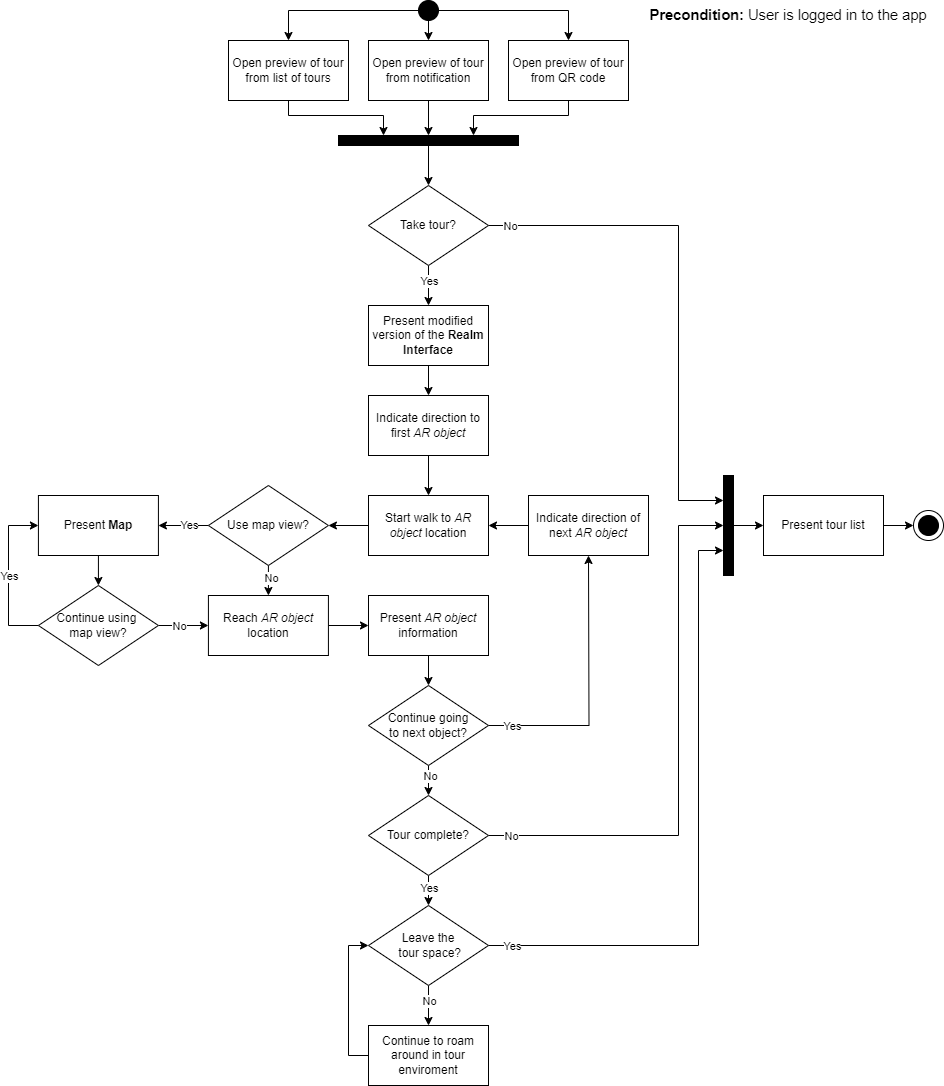
\includegraphics[scale=0.4]{SequenceDiagrams/UC4.png}\\ 
    \textbf{Figure 2: UC4}
\end{center}

\begin{center}
    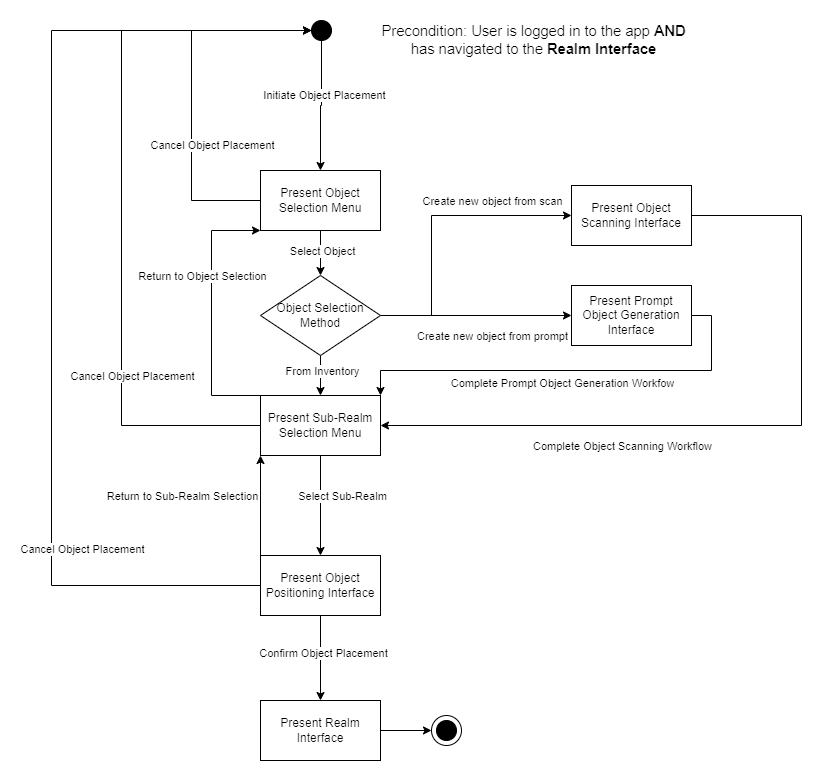
\includegraphics[scale=0.4]{SequenceDiagrams/uc7.png}\\ 
    \textbf{Figure 3: UC7}
\end{center}



\end{document}
